\documentclass[tikz,border=2pt]{standalone}
\usepackage{amsmath,amssymb}
\usepackage{pgfplots}
\pgfplotsset{compat=1.18}

\begin{document}
% Geometric probabilities p(1-p)^k with p = 1/4: each bar is 3/4 of the previous one, and the
% running total 1 - (3/4)^{k+1} approaches 1.
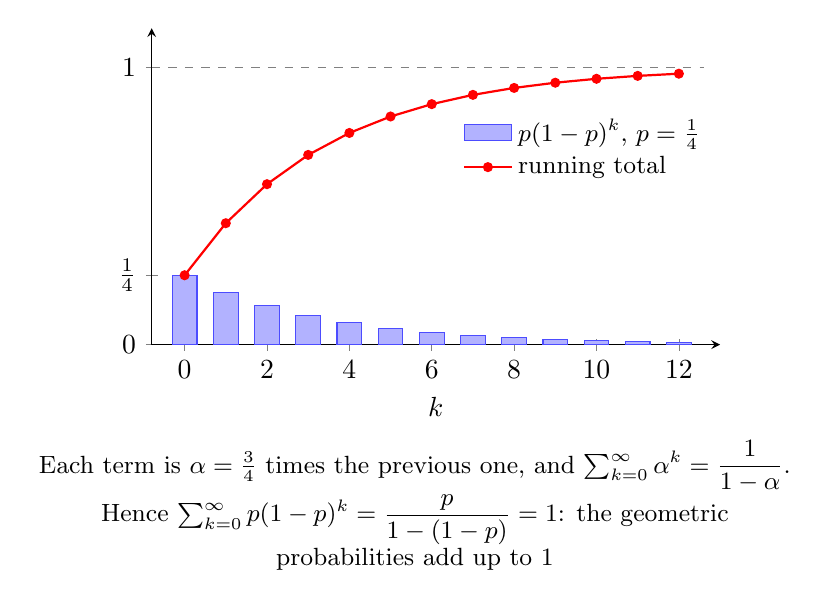
\begin{tikzpicture}
	\begin{axis}[
		axis lines=left, xmin=-0.8, xmax=13, ymin=0, ymax=1.14,
		xtick={0,2,4,6,8,10,12}, ytick={0,0.25,1}, yticklabels={$0$,$\tfrac14$,$1$},
		xlabel={$k$},
		width=8.8cm, height=5.6cm, clip=false,
		legend style={draw=none, fill=none, font=\small, at={(0.99,0.62)}, anchor=east}, legend cell align=left
		]
		\addplot[ybar, bar width=0.6, fill=blue!30, draw=blue!70, area legend] coordinates {(0,0.25) (1,0.1875) (2,0.1406) (3,0.1055) (4,0.0791) (5,0.0593) (6,0.0445) (7,0.0334) (8,0.0250) (9,0.0188) (10,0.0141) (11,0.0106) (12,0.0079)};
		\addlegendentry{$p(1-p)^k$, $p=\tfrac14$}
		\addplot[red, thick, mark=*, mark size=1.4pt] coordinates {(0,0.25) (1,0.4375) (2,0.5781) (3,0.6836) (4,0.7627) (5,0.8220) (6,0.8665) (7,0.8999) (8,0.9249) (9,0.9437) (10,0.9578) (11,0.9683) (12,0.9762)};
		\addlegendentry{running total}
		\draw[gray, dashed] (axis cs:-0.8,1) -- (axis cs:12.6,1);
	\end{axis}
	\node[anchor=north, font=\small, align=flush center, text width=9.6cm] at ([yshift=-2pt]current axis.outer south) {Each term is $\alpha=\tfrac34$ times the previous one, and $\sum_{k=0}^{\infty}\alpha^k=\dfrac1{1-\alpha}$. Hence $\sum_{k=0}^{\infty}p(1-p)^k=\dfrac p{1-(1-p)}=1$: the geometric probabilities add up to $1$};
\end{tikzpicture}
\end{document}
